\documentclass{llncs}

\usepackage{pslatex}
\usepackage{url}
\usepackage{latexsym}
\usepackage{alltt,verbatim,graphicx,xcolor}
\usepackage{amsmath,amssymb,url}

\newcommand{\ecal}{\mathcal{E}}
\newcommand{\rcal}{\mathcal{R}}
\newcommand{\tcal}{\mathcal{T}}
\newcommand{\rews}{\rightarrow}
\newenvironment{code2}{\begin{verbatim}}{\end{verbatim}}

\newcommand{\ignore}[1]{}
\newcommand{\tcode}[1]{\text{\tt #1}}
\newcommand{\obj}[1]{\langle \tcode{#1} \rangle}

\newcommand{\paco}[1]{\textcolor{red}{[Paco writes: #1]}}
\newcommand{\camilo}[1]{\textcolor{blue}{[Camilo writes: #1]}}


\title{Towards a Maude Formal Environment}

\author{Francisco Dur\'an\inst{1} \and Camilo Rocha\inst{2} \and Jos\'e M. \'Alvarez\inst{1}}

\institute{
Universidad de M\'alaga, Spain. %\email{duran@lcc.uma.es} 
\and
University of Illinois at Urbana-Champaign, IL, USA. %\email{meseguer@uiuc.edu}
}

%
% Margin notes
%
\newcounter{marginalnote}
\setcounter{marginalnote}{1}
\renewcommand{\themarginalnote}{\arabic{marginalnote}}
	
\setlength{\marginparwidth}{3cm}
	
\newcommand{\mnote}[1]
{\raisebox{1ex}{\scriptsize (\themarginalnote)}%
\marginpar{\footnotesize\raggedright\indent
\raisebox{1ex}{\scriptsize (\themarginalnote)} %\textcolor{red}
                                               {#1}}%
\addtocounter{marginalnote}{1}}
%


\begin{document}

\maketitle

\begin{abstract}
Maude is a declarative and reflective language based on rewriting
logic in which computation corresponds to efficient deduction by
rewriting. Because of its reflective capabilities, Maude has been
useful as a {\em metatool}
in the development of formal analysis tools for checking
specific properties of Maude specifications.
This includes tools for checking termination, confluence, and inductive
properties of rewrite theories. 
Nevertheless, most of these tools have been designed to work
in isolation, making it difficult, for instance, to exchange data between
them and inconvenient to switch between their environments.
This paper presents the Maude Formal Environment (MFE), 
an executable formal specification in Maude within which a 
user can interact with tools to mechanically verify 
properties of Maude specifications. 
One important aspect of this work is that the MFE 
has been designed to be easily extended with
tools having highly heterogeneous designs whilst creating
synergy among them. As a proof of concept,
we report on the integration of five 
commonly used formal analysis tools for Maude specifications into MFE
and illustrate their interoperability with an example.

%Besides giving support to exchange data among tools and
%to easily switch between their environments,\mnote{I whole emphasize on the interaction between the tools and in the holistic use in the environment (in the sense that they working together represents more than their sum.} 
%MFE also provides a new mechanism
%for recording user sessions\mnote{for me this is less relevant} and for maintaining 
%several instances of tools\mnote{I should leave this for the body of the paper as well}.

\end{abstract}


\section{Introduction}
\label{sec.intro}

There is a great deal of interest today in developing
multipurpose environments that combine declarative
programming with specification languages and useful
formal analysis tools (see, e.g., \cite{Mossakowski-Maeder-Luttich:2007,Franssen-Brand:2009,Hemer-Long-Strooper:2005,uitp-web-page,Aspinall-Luth:2007}).
Maude~\cite{CDELMMQ:2002,CDELMMT:2007-book} is a reflective declarative language and system based on 
rewriting logic in which computation
corresponds to efficient deduction by rewriting.
Maude has been successfully used as a {\em metatool} in the creation of tools for
verifying properties of Maude specifications~\cite{clavel99,CDHLMO:2007}.
Nevertheless, these tools work in isolation, 
making it inconvenient to switch between their environments
and difficult to exchange data between them.
In this sense, despite its title, previous work presented in~\cite{CDHLMO:2007}
does not conform to the notion of formal tool environment discussed here.
In response to these limitations, 
we present the Maude Formal Environment (MFE),
an executable and highly extensible software infrastructure
within which a user can interact with several 
tools to mechanically verify properties of Maude specifications.
In MFE, tool interoperability allows for discharging proof obligations
of different nature without switching between different
tool environments.
The integration of different tools inside 
MFE's common environment presents the user with a consistent user interface,
a mechanism to keep track of pending proof obligations,
and allows the execution of several instances of each tool,
among other features.

%One of the key aspects to designing a
%formal environment is to identify what its {\em purpose} is.
%Once this aspect is clear, there is one important implementation 
%question to answer: 
%what {\em model} to chose so that it is flexible enough to accommodate 
%existing tools and extensible enough to facilitate
%future developments? 
The purpose of MFE is to
support interactive formal analysis of Maude specifications,
and therefore the integration of tools within MFE 
revolves around Maude modules.
MFE is naturally modeled in Maude as an object-based system in which the tools are 
objects and their communication mechanism
is message passing. User interaction is available through
Full Maude~\cite{Duran-Meseguer:2007-scp,CDELMMT:2007-book}, an extension of Maude that
has become a common base on top of which tools
can be built, offering a modular design for easily
integrating other tools written in Maude (see, e.g.,~\cite{Duran-Olveczky:2008-wrla} for a guide on how to extend Full Maude).

One of the most interesting challenges was to make the 
MFE design highly extensible and amenable to tool interoperability.
In MFE, there is no constraint on how each tool 
should model its particular domain or how it maintains its internal
state. We implemented an object-based version of the 
{\em model-view-controller} 
pattern to separate the modeling of the domain for each tool,
the presentation of information, and the actions based on user input
into separate objects. 
This pattern isolates the application logic for the user from the 
user input and presentation, permitting independent development, 
testing and maintenance of each.
We also followed
good object-oriented design practices that kept the
cohesion high and the coupling low among objects.
In our experience, these good design practices proved
key for the integration of tools
in MFE.

We report here on the integration of five tools 
with highly different designs and implementations in MFE. Namely, 
the Maude Termination Tool (MTT)~\cite{Duran-Lucas-Meseguer:2008-ijcar},
the Church-Rosser Checker (CRC)~\cite{Duran-Meseguer:2010-wrla-crc,Duran-Meseguer:2011},
the Coherence Checker (ChC)~\cite{Duran-Meseguer:2010-wrla-chc,Duran-Meseguer:2011},
the Sufficient Completeness Checker (SCC)~\cite{Hendrix-Clavel-Meseguer:05,Hendrix-Meseguer-Ohsaki:2006},
and Maude's Inductive Theorem Prover (ITP)~\cite{Clavel-Palomino-Riesco:2006,Hendrix:2008}.
Despite their heterogeneousness and isolated conception,
these tools were integrated in MFE with very few code alterations,
many of these due to renaming of sorts and operators.
For tools which depend on external
utilities not directly available from Maude such as MTT and SCC, 
we have extended the Maude system to a non-official distribution
with {\em built-in} operators associated with appropriate
C++ code that interacts with the external tools.
A similar extension was already performed for SCC~\cite{Hendrix:2008}.

%\camilo{Paco, qu\'e te parece si eliminamos este p\'arrafo?}
%The task of proving formal properties of 
%software specifications needs valuable human effort
%and hence, there is a great interest in building libraries
%of completed theorems (see, e.g., \cite{Aspinall-Luth-Winterstein:2007,Franssen:2010}). For a first effort in this 
%direction, MFE adds support for automatically 
%storing user sessions to enable re-use. Within
%a session, the user can instantiate a tool 
%with as many goals as necessary, send requests
%from one tool to another, and even rely on external
%tools to handle proof obligations. 

MFE, with these five tools, as well
as some examples and some preliminary documentation, is available
at \url{http://maude.lcc.uma.es/MFE}.

\paragraph{\bf Outline of the paper.} 
Section~\ref{sec.prelim} gives a summarized account
of Maude's object-based programing and support for user interoperability.
Section~\ref{sec.design} discusses the main design
aspects of MFE. 
Section~\ref{sec.tools} describes the tools available
from the current version of MFE.
Section~\ref{sec.extend} illustrates how to extend MFE with a concrete tool 
and Section~\ref{sec.example} presents
a case study in which a user interacts with several tools 
within MFE.
Finally, Section~\ref{sec.concl} presents related and future work,
and some concluding remarks.

\section{Object-Based Programming and User Interfaces in Maude}
\label{sec.prelim}

We assume that the reader is familiar with the basics of rewriting
logic and Maude, and refer to~\cite{CDELMMT:2007-book} for 
an introduction to these.

Maude can be used not only to define domain-specific languages
or tools, but also to build environments for such languages and tools.
In such applications, the predefined $\tcode{LOOP-MODE}$ module can 
be used to handle
the input/output and to maintain the persistent state of the language
environment or tool. This section explains some basic background on how
object-based systems, which naturally model distributed systems in Maude,
and the $\tcode{LOOP-MODE}$ module are used to define MFE's 
interactive infrastructure as an extension of Full Maude.

\paragraph{\bf Object-based programming.}
Maude supports the modeling of object-based systems in the
predefined $\tcode{CONFIGURATION}$ module that declares sorts
representing the essential concepts of object, message, and
configuration, along with notation for object syntax that serves
as a common language for specific object-based systems. 
The basic sorts defined in \tcode{CONFIGURATION} are \tcode{Object},
\tcode{Msg}, and \tcode{Configuration}. A configuration is
a multiset of objects and messages that represent a possible system state.
Configurations are formed by multiset union, represented by empty syntax \verb~__~,
starting from singleton objects and messages.
The empty configuration is represented by the constant \tcode{none}. 

%A typical configuration has the form 

%\begin{alltt}
%\(\obj{Ob\({}_{1}\)} \dots \obj{Ob-m} \obj{Mes-1} \dots \obj{Mes-n}\)
%\end{alltt}

%where $\obj{Ob-1} \dots \obj{Ob-m}$ are objects,
%$\obj{Mes-1} \dots \obj{Mes-n}$ are messages, and the order is immaterial.

\begin{small}
\begin{verbatim}
  sort Configuration .
  subsorts Object Message < Configuration .
  op none : -> Configuration [ctor] .
  op __ : Configuration Configuration -> Configuration
      [ctor assoc comm id: none] .
\end{verbatim}
\end{small}
%
In general, a rewrite rule for an object-based system has the form

{\small \ttfamily
\begin{tabbing}
\     \ cr\=l [\textit{r}] :\\
      \> \(\textit{Obj}_1\;\ldots\;\textit{Obj}_m\;\textit{Msg}_1\;\ldots\;\textit{Msg}_n\) \\
      \> => \= \(\textit{Obj}'_1\;\ldots\;\textit{Obj}'_j\;\textit{Obj}_{m+1}\;\ldots\;\textit{Obj}_p\;\textit{Msg}'_1\;\ldots\;\textit{Msg}'_q\) \\
      \> if \textit{Cond} .
\end{tabbing}
\rmfamily }

%\begin{alltt}
%rl \(Ob_{1} \dots \obj{Ob-m} \obj{Mes-1} \dots \obj{Mes-n}\)
%=> \(\obj{Ob'-1} \dots \obj{Ob'-j} \obj{Ob-m+1} \dots \obj{Ob-p} \obj{Mes'-1} \dots \obj{Mes'-q}\; .\)
%\end{alltt}

\noindent where objects \texttt{\(\textit{Obj}'_1 \ldots \textit{Obj}'_j\)} are updated versions of objects
\texttt{\(\textit{Obj}_1 \ldots \textit{Obj}_m\)}, for $j \leq m$, 
\texttt{\(\textit{Obj}_{m+1} \ldots \textit{Obj}_p\)} are newly created objects,
\texttt{\(\textit{Msg}_1 \ldots \textit{Msg}_n\)} are consumed messages, 
and \texttt{\(\textit{Msg}'_1 \ldots \textit{Msg}'_q\)} are new messages.

The user is free to define any object or message syntax that is convenient.
However, for uniformity in identifying objects and message receivers,
the adopted convention is that {\em the first argument of an object constructor should be its identifier}, and {\em the first argument of a
message constructor should be the identifier of its addressee}. Module $\tcode{CONFIGURATION}$
provides an object syntax that serves as a common notation that can be used by
developers of object-based system specifications, as is the case
in Full Maude. This module introduces sorts $\tcode{Oid}$ for
object identifiers, $\tcode{Cid}$ for class identifiers,
$\tcode{Attribute}$ for named elements of an object's state,
and $\tcode{AttributeSet}$ for multisets of attributes. 
In this syntax, objects have the general form
\texttt{\(\texttt{<} \; \textit{O} \; \texttt{:} \; \textit{C} \; \texttt{|} \; \textit{a}_1 \texttt{:} \textit{v}_1
\texttt{,} \; ... \texttt{,} \; \textit{a}_n \texttt{:} \textit{v}_n \; \texttt{>}\)}
%\begin{alltt}
%< O : C | \(\obj{att-1} \dots \obj{att-k}\) >
%\end{alltt}
where \texttt{\textit{O}} is an object identifier, \texttt{\textit{C}} is a class identifier, and 
the \texttt{\(\textit{a}_i \texttt{:} \textit{v}_i\)} are 
pairs of an attribute name $\textit{a}_i$ and a value $\textit{v}_i$, for $1\leq i\leq n$. 

%are the object's attributes. Attribute sets
%are formed from singleton attributes by a multiset union operator $\_,\_$
%with identity $\tcode{none}$, the empty multiset.

Full Maude provides convenient notation for object-oriented modules in which classes are declared with
the syntax 
{\small \ttfamily
\begin{tabbing}
\ \ class \textit{C} | \(\textit{a}_1\) : \(\textit{S}_1\), ..., \(\textit{a}_n\) : \(\textit{S}_n\) .
\end{tabbing}
\rmfamily}
\noindent where \texttt{\textit{C}} is the name of the class,
the \texttt{\(\textit{a}_i\)} are attribute identifiers, and the \texttt{\(\textit{S}_i\)} are the sorts of the corresponding
attributes. Class inheritance is directly supported by Maude's order-sorted type structure.
A subclass declaration
{\small
\begin{alltt}
  subclass \textit{C} < \textit{C}' .
\end{alltt}
}
\noindent is just a particular case of a subsort
declaration \texttt{\(\textit{C}\) < \(\textit{C}\)'}. The effect of a subclass declaration is that the attributes,
messages, and rules of all the superclasses, together with the newly defined
attributes, messages, and rules of the subclass, characterize the structure and
behavior of the objects in the subclass.
In what follows, we use this convenient object-oriented notation for defining classes.
See~\cite{CDELMMT:2007-book} for further details on this notation and on the 
transformation of object-oriented modules into system modules. 

\paragraph{\bf User interfaces.}
Module $\tcode{LOOP-MODE}$ specifies in Maude
a general input/output facility by a read-eval-print loop
using object-based concepts.
A {\em loop object} is a term of the form \verb~[In,St,Out]~ where
\verb~In~ is an input stream, \verb~Out~ is an output stream, and 
\verb~St~ is its state. 
%Operator
%\begin{alltt}
%op [_,_,_] : QidList State QidList -> System [...] .
%\end{alltt}
%can be seen as an object, called the {\em loop object}, with an input
%stream (the first argument), an output stream (the third argument), and
%a state (given by the second argument). 
%In the current release only
%one input stream is supported (the current terminal). 
One can think
of the input and output events as implicit {\em rewrites} that transfer
the input and output data between two objects, namely the loop object
and the user (or terminal) object.

Loop objects are constructed with the operator 
\begin{verbatim}
  op [_,_,_] : QidList State QidList -> System [...] .
\end{verbatim}
Besides having input and output streams,
terms of sort $\tcode{System}$ give a generic way for maintaining a state
in its second component. In fact, sort $\tcode{State}$ in
$\tcode{LOOP-MODE}$ does not have any constructors, giving complete
flexibility for defining the terms we want to have for representing
the state of the loop. In MFE, we represent state terms as
configurations of objects and messages, by declaring sort {\tt Configuration}
as subsort of {\tt State}.

Rewrite rules define the interaction of the state with the loop
and the changes produced in the state by the actions requested by the user.
In order to generate in Maude an {\em interface} for interacting with an application,
the language for interaction needs to be defined by a data type for commands and other constructs.
In this way, a rule can detect when a valid request has been introduced
by the user, and if the state of the system allows it, passes it as the next
action to be attempted. For the other direction of interaction, a rule
detects when the state has a response to be output and, in that case, 
it places it in the output component of the loop object.

\paragraph{\bf Full Maude.}
In Full Maude, the persistent state of the read-eval-print loop
 provided by module
\texttt{LOOP-MODE} is given by a single object of class 
\texttt{DatabaseClass}. 
%
Objects of this class have: an attribute \texttt{db} of sort 
\texttt{Database} to keep the actual database where all the
modules entered to the system are stored,
an attribute \texttt{default} denoting the name of the current 
default module, and attributes \texttt{input} and \texttt{output}
that simplify the communication between the read-eval-print loop 
and the database object. 
%
Using the above syntactic sugar for object-oriented modules, 
we can declare such a class as:

\begin{small}
\begin{verbatim}
 class DatabaseClass | 
   db : Database, default : ModName, input : TermList, output : QidList .
\end{verbatim}
\end{small}
%
Inputs from the user into Full Maude are parsed using the built-in \texttt{metaParse} function. For such parsing, Full Maude uses
the \texttt{FULL-MAUDE-SIGN} module, in which we can find the 
declarations so that any valid input can be parsed. 
In particular, we find in these modules, among others, sorts 
\verb~@Module@~, 
\verb~@ModExp@~, 
and \verb~@Command@~, of modules, 
module expressions, and commands, respectively,
and syntax declarations such as:

\begin{small}
\begin{verbatim}
 op select_. : @ModExp@ -> @Command@ .
 op show module_. : @ModExp@ -> @Command@ .
 op mod_is_endm : @Interface@ @SDeclList@ -> @Module@ .
 op omod_is_endom : @Interface@ @ODeclList@ -> @Module@ .
\end{verbatim}
\end{small}
%
for commands
\texttt{select} and \texttt{show module}, and for system and object-oriented modules. 

The behavior of Full Maude upon the reception of new inputs from the user is specified by rewrite rules. For the different commands, different actions are accomplished. 

\section{The Design of MFE}
\label{sec.design}

The object-oriented model of MFE consists of three classes: 
the class \texttt{Proof} of proof objects that keep the state of specific proof requests,
the class \texttt{Tool} of tool objects that manage proof objects, and
a class \texttt{Controller}
that inherits from the Full Maude's \texttt{DatabaseClass} 
and provides a centralized entry point for 
handling requests to the formal environment.

The \texttt{Controller} object orchestrates the behavior of the 
environment with the user and of the environment 
with its tools. 
The user interacts with the environment via commands
that are encapsulated as messages in the object configuration. Each
tool object and the controller object have a module defining 
the grammar of the commands it can handle. 
The controller handles any command it can parse;
since this object extends Full Maude, it handles its own commands
and Full Maude ones.
If the controller receives a command it cannot parse, it
will delegate it to the current {\em active} tool. 
If the active tool can parse the delegated command, 
then it notifies the controller and handles the command.
Otherwise, it notifies the failure to the controller
that in turn will notify the failure to the requester.

Classes \texttt{Proof} and \texttt{Tool} define some basic 
functionality for tools and, as we will see in 
Section~\ref{sec.extend} for a sample tool,  
are provided to simplify the task of 
incorporating new tools to the environment. 
However, tools can be added to the environment by 
defining the expected interaction with the controller object 
without using classes \texttt{Proof} and \texttt{Tool}. This was 
the case, for example, with the ITP tool that does not use in MFE the 
infrastructure provided by classes \texttt{Proof} and \texttt{Tool}.

In the following subsections we describe in more detail 
the object-based model of MFE and its interaction mechanism.

\subsection{Proof Objects}

Proof objects maintain 
the state of specific proof requests to a tool object. 
Every proof object maintains
in its state the information of the module associated to the proof obligation
and a set of object identifiers corresponding to the objects 
submitting the proof obligation. 

\begin{small}
\begin{verbatim}
  class Proof | module : Module, requester : Set{Oid} .
\end{verbatim}
\end{small}
%
The concept of a proof object representing the state of
a proof requirement, is key for enabling tools 
in MFE with support for 
multiple proof requirements. Namely, handling a ``new
proof'' command corresponds to instantiating a proof object
with the appropriate attribute data. 
Commands that incrementally modify the status of a proof
obligation result in updates to the attributes of the proof
object.
For example, a CRC proof object will keep track of confluence and/or 
sort-decreasingness checks, and will be updated every time a new proof 
obligation is discharged; when all proof obligations have been proved, 
it will realize the check's completion and will inform all its requesters. 

A subclass of \texttt{Proof} may be defined
for each tool in the environment, adding the additional attributes and 
behavior required by the specific tool.  
Proof obligation objects, for instance, can be extended with
additional attributes for keeping track of dependencies
of subgoals that should be handled by other tools, timeouts, number of attempts, 
or any other required information.

\subsection{Tool Objects}

A tool object is responsible for maintaining the life cycle of
its proof objects. When a tool object receives a request for a new proof,
it tries to create a new proof object for it and, if successful, 
it sets the new proof object
as active so that any command from the user or message from other 
tools in the environment are forwarded to it. 
There is exactly one tool object
for each tool in the formal environment. 

Every tool object
has an attribute \texttt{grammar} that defines the grammar of user commands
the tool can handle.
Tools may rely on other tools, hence a tool object has
attribute \texttt{tools} with a map from tool names to the object identifiers of the corresponding tools in the environment. If proof obligations are due, this attribute will be used to submit them to the appropriate tools. 
The references of proof objects associated to a tool object are
maintained with a map from module names to object identifiers in attribute \texttt{reg}.
In MFE, a tool may perform several analyses on a module, so
that the information of such analyses is kept in the
attributes of the corresponding proof object.
A tool object also keeps in attribute \texttt{current} 
a reference to one of its proof
objects, if any, which is referred by the tool as its {\em active}
proof obligation.

\begin{small}
\begin{verbatim}
  class Tool | grammar : Module, 
               tools : Map{ToolName, Oid}, 
               reg : Map{ModuleName, Oid}, 
               current : Oid, 
               index : Nat .
\end{verbatim}
\end{small}
%
Integration and interoperability of tools within MFE revolves around modules, and therefore, typically, the ``new goal'' commands 
have a module expression as parameter, although in general commands
may have other parameters. For example, a check of the Church-Rosser property would take just the module to be checked as parameter.
However, one can perform checks of coherence in the coherence checker with the option of checking coherence or ground coherence via an additional parameter. 
The decision of whether a new proof object is generated or not for a module when attempting different kinds of checks is up to the tool developer. 

Despite this flexibility, in the general approach a tool object will create a new proof object for a module $M$ whenever there is no record of $M$ being previously handled by the tool, namely, if name of module $M$ is not in the domain of the {\tt reg} attribute. More precisely, when a proof is requested, the \texttt{reg} attribute is checked: if there is a proof for a module with such a name, then the module itself is compared with the current one, to make sure that the module has not changed. In case there is some parameter, as for example an alternative transformation for a termination proof, if the proof has not succeeded before then the check is attempted: the existing proof object is replaced with the one corresponding to the new proof. 

The different tools may perform tool specific checks on a parameter module $M$ and if these checks succeed, then a new proof 
object is instantiated with a unique object identifier, with $M$ as associated module (in attribute {\tt module}), and the corresponding
reference of the requesting object (in attribute \texttt{requester}). 
The remaining attributes of the proof
object are set according to the purpose
of the tool. 
%Additionally, the registry {\tt reg},
%the active proof object {\tt current}, and counter {\tt index}
%attributes are updated accordingly. 
%A tool object may send some messages, for instance, to the user
%or to other tools.

See Section~\ref{sec.extend} for an example of this behavior in the case of SCC. %the Sufficient Completeness Checker.

%{\small
%\begin{verbatim}
%crl [check] :
%   < O : Tool | reg : MNReg, current: O'', index: N, Atts > 
%   (to O from O' : check M)
%=> < O : Tool | reg : (MNReg, M |-> s(N)), current: po(s(N)), index: s(N), Atts >
%   < po(s(N)) : Goal | module : M, requester : O', processAttributes(M) >
%   processMessages(O',O,...)
%if not getName(M) in domain of MNReg 
%/\ admisibleModule(M) .
%\end{verbatim}
%}

\subsection{The Controller Object}

The task of the controller object is twofold: it provides a centralized
entry point for handling user requests 
and it manages the tools that are available in the environment.

The \texttt{Controller} class inherits from Full Maude's \texttt{DatabaseClass}, 
and in addition to its module database and all the functionality for handling 
all Full Maude commands, the controller object stores information on
the tools available in MFE. This is achieved by using the attribute
{\tt tools} that is a map from tool names into object identifiers.
In the attribute {\tt current-tool} the controller object maintains a 
reference to the active tool:

\begin{small}
\begin{verbatim}
  class Controller | current-tool : Oid, tools : Map{ToolName, Oid} .
  subclass Controller < DatabaseClass .
\end{verbatim}
\end{small}
%
The controller object is {\em the singleton} instance {\tt mfe} of
class {\tt Controller}.
To handle a command, the object \texttt{mfe} first tries using its
grammar (which extends that of Full Maude). If the command
can be parsed with its grammar, then \texttt{mfe} handles
the request. Otherwise, it delegates the command to the 
active tool and waits for an answer.
The user can select the active tool via a ``select'' command.
The answer to the delegated request can be either affirmative or not,
meaning that the tool can parse the command and will
handle it, or that the given command does not conform to the grammar
and therefore cannot be handled by the tool.
Because of the way user and tool interaction has been designed and
implemented in MFE, there is no need to enforce a policy of
uniqueness of commands among its tools: if two tools share
a command syntax, then such command will be handled by the controller
object or else by the active tool. This simplifies the integration of
existing tools, because most of their implementations can directly be used 
and because all proof scripts available are still usable after adding 
the appropriate selection and submission commands. 

The \verb~Controller~ class adds the following commands to those available in Full Maude:
\begin{description}
\item[\verb~(select tool <tool-name> .)~] sets the tool \verb~<tool-name>~ as active tool.
\item[\verb~(MFE help .)~] shows information on the commands available.
\item[\verb~(show global state .)~] shows the state of the framework.
\end{description}
%
To illustrate the way in which the behavior of the controller object works, we present the
{\tt select-tool} rewrite rule that implements tool selection in MFE for the
controller:
%\newline
%{\small
%%\begin{verbatim}
%\verb~  (select tool <tool-name> .)~
%%\end{verbatim}
%}
%\newline
%%\noindent 
% in MFE. %, which takes as parameter the name of a tool.

\begin{small}
\begin{verbatim}
 var X@Controller : Controller .   var Ct : Constant .       
 var TS : Map{ToolName, Oid} .     var QIL : QidList .       
 var Atts : AttributeSet .         var O : Oid .  
   
 crl [select-tool] :
    < mfe : X@Controller | input : ('select`tool_.[Ct]), 
       output : QIL, 
       current-tool : O, 
       tools : TOOLS, 
       Atts >
    => < mfe : X@Controller | input : nilTermList, 
          output : QIL 'The getName(Ct) 'has 'been 'set 'as 'active 'tool., 
          current-tool : TOOLS[qid2tool(getName(Ct))], 
          tools : TOOLS, 
          Atts > 
    if TOOLS[qid2tool(getName(Ct))] =/= null .
\end{verbatim}
\end{small}
%
When the result of parsing a ``select tool'' command in the grammar of the controller is placed 
in the \texttt{input} attribute of the \texttt{mfe} object, and it corresponds to a tool in
the environment (see the condition in rule \texttt{select-tool}),
then such a tool is set as the active one. Functions \texttt{getName} and \texttt{qid2tool} 
return the name of a given constant and transforms a quoted identifier into a tool name, respectively. 
A second rule (omitted here) handles the case in which the argument of the select command 
does not correspond to a tool in the environment; this rule reports on 
the situation by creating an error message.

\subsection{User Interaction and Tool Interoperability}

In the object configuration of MFE, user interaction is achieved via commands
and tool interoperability via messages. Upon successful parsing, commands 
are converted into messages. With this approach, requests from users and from 
tools are handled in a uniform manner by just distinguishing the requester. 

MFE internal messages identify their contents with ``to-from''
information and name the different operations offered by 
the tools and their answers.
% and are of two types depending on their contents.
%A {\em parsing message} is a message having as contents 
%the meta-representation of an user command. 
%An (MFE) {\em internal message} is a message
%that corresponds to the commands available from
%each tool in  the formal environment. 
%The following is the syntax of messages in MFE:
Using the following syntax for messages, each tool defines 
its corresponding message bodies.

\begin{small}
\begin{verbatim}
  sort MFEMsgBody .
  op to_from_:_ : Oid Oid MFEMsgBody -> Msg [ctor] .
\end{verbatim}
\end{small}
%
If a user command parses in the controller's grammar, then the controller handles the command.
If it fails, then the input is submitted to the active tool.
The tool is expected to return an ``input parsed'' message indicating whether or not
it is able to parse the command or not. Rewrite rule {\tt input}, below,
defines the behavior of a tool object that is able to parse the
input command. Observe that when a tool object can parse
a command, it sends two messages. Namely, it creates a copy of
the original message but with a parsed version 
of the input command and it sends the requester an output message
indicating that the input can be parsed.

\begin{small}
\begin{verbatim}
  var  X@Tool : Tool .               vars  O O' : Oid .
  var  Atts : AttributeSet .         var  QIL : QidList .
  var  G : Module .
 
 crl [input] :
    < O : X@Tool | grammar : G, Atts >
    (to O from O' : input(QIL))
    => < O : X@Tool | grammar : G, Atts >
       (to O from O' : getTerm(metaParse(G, QIL, '@Input@)))
       (to O' from O : input-parsed(QIL, true))
    if RP:ResultPair := metaParse(G, QIL, '@Input@) .
\end{verbatim}
\end{small}
%
If the tool cannot parse the input, then another rule (omitted here)
sends the requester an \texttt{input-parsed} message with its second argument 
set to \texttt{false}. When the controller receives the \texttt{input-parsed} 
message, with \texttt{true} or \texttt{false}, it proceeds either by letting 
the corresponding tool resolve the command or by displaying an error 
message. 

\section{Tools in MFE}
\label{sec.tools}

Five formal analysis tools are available 
in the current release of MFE.
The Maude Termination Tool (MTT) can be used
to prove termination of functional and
system modules, the Church-Rosser Checker (CRC)
can be used to check the Church-Rosser property 
of functional modules, the Coherence Checker (ChC)
can be used to check the coherence of system modules,
the Inductive Theorem Prover (ITP) can be used to verify 
inductive properties of functional modules, and
the Sufficient Completeness Checker (SCC) can
be used to check completeness of functional modules
and deadlock freedom of system modules.
One important aspect in the integration task
is the interaction complexity due to the nontrivial 
dependencies among tools. Figure~\ref{fig.tool-dep}
depicts the tool-dependency graph for these five tools.

\begin{figure}[htbp]
\begin{center}
%\fbox{
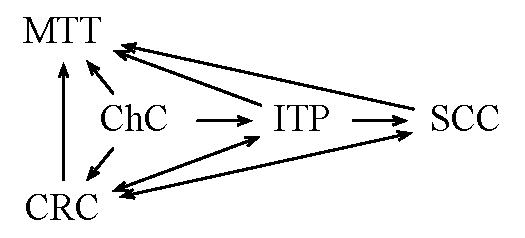
\includegraphics[width=5cm]{tool-dep}
%}
\caption{Tool-dependency graph in MFE.}
\label{fig.tool-dep}
\end{center}
\end{figure}

In the following paragraphs 
we summarize the main features
and dependencies of the five tools available in MFE. 
For further details on these tools, including user
manuals, restrictions, and examples, we refer the reader
to the given references and web sites.

\subsection{The Maude Termination Tool}
\label{sec.mtt}


Maude has expressive features including advanced typing constructs
with sorts, subsorts, kinds, and memberships; matching modulo axioms;
evaluation strategies for both equations and rewrite rules; and very 
general conditional equations and rewrite rules. Proving termination
of programs having such features is nontrivial. Furthermore, some of
these features are not supported by standard termination methods and
tools. Yet, the use of such features may be essential to ensure termination.
MTT uses several non-termination preserving theory 
transformations~\cite{Duran-Lucas-Meseguer:2009-prole,Duran-Lucas-Meseguer:2009-frocos}
which are applied in a kind of pipeline to a module $M$, obtaining
a module $M'$ in such a way that a proof termination of 
$M'$ witnesses the termination of $M$. For instance, 
by sequentially using four theory transformations,
a conditional order-sorted context-sensitive system module 
can be transformed into an unconditional unsorted
context-sensitive term rewrite system, which can be 
handled by the back-end tools.

The Maude Termination Tool (MTT) is a tool that checks the
termination of (possibly conditional) order-sorted
Maude functional or system modules. 
The current implementation takes a module
as input and tries to prove its termination by applying 
{theory transformations} and then invoking back-end termination tools,
such as MU-TERM~\cite{Lucas:2004} and AProVE~\cite{Giesl-Schneider-Kamp-Thiemann:2006}, that can prove termination of (variants of) rewriting.
For the current version of MFE, a new ``hook'' to a C++
library was included in non-official distribution of
Core Maude for invoking these back-end termination tools.
MTT is the only tool in the MFE
that does not depend on any other tool in the environment.

A stand-alone version of MTT, with a graphical user interface,
is available from \url{http://www.lcc.uma.es/~duran/MTT/}.

\subsection{The Church-Rosser Checker}
\label{sec.crc}

The Church-Rosser Checker (CRC) checks the
Church-Rosser property of Maude functional (possibly conditional)
order-sorted modules. For order-sorted modules, being Church-Rosser
and terminating means not only confluence, but also a 
{sort-decreasingness} property: each normal form has the least possible
sort among those of all equivalent terms.
CRC depends on MTT for checking termination assumptions
and on ITP for inductive theorem proving (see Section~\ref{sec.itp}).
Some of the proof obligations are not currently 
handled by any tool. We will se in Section~\ref{sec.example} that 
although they are submitted to ITP, these proofs may be ``trusted'' by the user.

CRC can be used to check equational specifications 
$(\Sigma,E\cup Ax)$ with an initial semantics that have already 
been proved terminating and need to be checked
(ground) Church-Rosser. The tool performs both a local confluence check
by computing all {\em (conditional) critical pairs} of the equations $E$
modulo the structural axioms $Ax$ 
%(i.e., overlaps among the left-hand sides of the equations in $E$ modulo $Ax$)
and a sort-decreasingness test in the form of membership assertions
for each equation in $E$ modulo $Ax$. If the 
(conditional) critical pairs or the sort decreasingness tests cannot
be discharged by CRC, proof obligations 
%consisting of a set of critical
%pairs and set of membership assertions that must be proven, respectively,
%(ground) joinable and (ground) reachable to a term with the required sort, 
are displayed as a guide to the user. In MFE, CRC can submit these
proof obligations to ITP for inductive
reasoning. 
%In other cases, the user may in
%fact have to modify the original specification by carefully considering the
%information conveyed by the proof obligations.

CRC, with its documentation and some examples, is available from
\url{http://maude.lcc.uma.es/CRChC/}.

\subsection{The Coherence Checker}
\label{sec.chc}

{\em (Ground) coherence} allows reducing the problem of computing rewrites of
the form $[t]_{E\cup Ax} \rews [t']_{E\cup Ax}$ that in general is
undecidable, to the much simpler and decidable problem of computing
rewrites of the form $[t]_{Ax} \rews [t']_{Ax}$, for $t$ and $t'$ 
any (ground) $\Sigma$-terms.
Intuitively, coherence means
that rewriting with $R$ modulo $E\cup Ax$ can be achieved by adopting
the strategy of first simplifying to canonical form with $E$ modulo $Ax$
and then applying a rule in $R$ modulo $Ax$.

The Coherence Checker (ChC) is a tool that provides a
(ground) coherence decision procedure for order-sorted system modules
$\rcal = (\Sigma,E\cup Ax,R)$. The tool calculates the set of
critical pairs between the equations $E$ and the rewrite rules $R$
modulo the structural axioms $Ax$, 
whose equational validity guarantees the (ground)
coherence of $\rcal$. ChC depends on MTT for termination
assumptions and on CRC for the equations $E$ being Church-Rosser.
Since this property is inductive, in some cases ITP can be used to
prove some proof obligations.

ChC, with its documentation and some examples, is available from
\url{http://maude.lcc.uma.es/CRChC/}.

\subsection{The Sufficient Completeness Checker}
\label{sec.scc}

Maude Sufficient Completeness Checker (SCC) is a tree automata based tool
for checking {\em sufficient completeness} and {\em deadlock
freedom} of terminating and sort-decreasing Maude modules.
Both sufficient completeness and deadlock freedom are relative
to {\em constructor} subsignatures.
For $\rcal=(\Sigma,E,R)$, a signature pair $(\Upsilon,\Omega)$,
with $\Upsilon \subseteq \Omega \subseteq \Sigma$, is a pair of
constructors for $\rcal$ if for each sort $s$ in $\Sigma$ and
each ground $\Sigma$-term with sort $s$, (i) there is a $\Omega$-ground term $u$
with sort $s$ satisfying the equality $t =u$ in $E$,
and (ii) there is a ground $\Upsilon$-term $v$ with sort $s$
satisfying the sequent $t \rightarrow v$ in $R$.
Intuitively, sufficient completeness is the
property that every operation in a specification
is equationally defined for all inputs, and
deadlock freedom is the property that every
nondeterministic computation leads to a terminal 
state~\cite{Rocha-Meseguer:2010,Hendrix:2008}.

Sufficient completeness and deadlock freedom are important properties both for developers 
of specifications, to check that they have not missed a case in defining
operations, and to inductive theorem provers, to check the soundness of
a proposed induction scheme. 
In the case of equational specifications, SCC assumes the 
input specification is ground sort-decreasing and terminating; 
in the case of rewrite specifications, SCC assumes the
input specification is ground sort-decreasing, terminating,
Church-Rosser, and coherent.

The tool is designed for unparameterized, order-sorted, left-linear, and 
unconditional Maude specifications that are ground terminating and Church-Rosser. 
It is a decision procedure for this class of specifications when every associative symbol 
is also commutative. For associative symbols that are not commutative it 
uses machine learning techniques that work well in practice. 
If the specification is not sufficiently complete, SCC returns a 
counterexample to aid the user in identifying errors. 
The tool is not complete for specifications with non-linear or 
conditional axioms, but nevertheless has proven useful in identifying 
errors in such specifications.
SCC accepts interactive commands to check the sufficient completeness of a Maude 
module, and internally constructs a propositional tree automaton whose language is 
empty if and only if the Maude module is sufficiently complete. The emptiness check is performed by 
a C++ tree automata library named CETA. 

The tool also supports several important completeness 
and freeness problems of context-sensitive specifications involving both equations
and rewrite rules~\cite{Rocha-Meseguer:2010,Hendrix:2008}.

SCC is available from its website at \url{http://maude.cs.uiuc.edu/tools/scc}.

\subsection{The Maude Inductive Theorem Prover}
\label{sec.itp}


The Maude Inductive Theorem Prover (ITP) is an experimental proof
assistant aiding in the task of proving inductive 
properties of the initial algebra 
associated to a membership equational theory. 
It is based on Membership Equational
Logic, a good fit for reasoning inductively about functions and
data structures involving partiality, subsorts, and conditions.
ITP supports proofs by structural induction and complete induction, 
in which operations need not be completely specified. Goals are either
conditional equations or conditional memberships, and inference steps are
available through a series of user commands.
ITP depends
on MTT for checking termination assumptions, on SCC
for checking sufficient completeness and freeness of equational
constructors, and on CRC for checking the Church-Rosser property
of the equations.

The ITP tool, documentation, and some examples are available from
\url{http://maude.cs.uiuc.edu/tools/itp/}.


\section{Extensibility by Example: the Integration of SCC}
\label{sec.extend}

In this section we present a brief overview of 
the steps undergone to integrate SCC in MFE.
In order to take as much advantage as possible
of the infrastructure offered by MFE, some classes offered by MFE
such as {\tt Tool} and {\tt Proof}
are specialized with new attributes and behavior specific to SCC. In this way,
SCC inherits the behavior defined already for these classes in MFE.
Internal messages defining SCC's public interface
are created and the rewrite rules defining SCC's behavior
are updated so they fit into MFE's message passing interaction mechanism.
Also, the controller object is modified 
to account for SCC in the object-based configuration of 
the formal environment.

\subsection{SCC Proof Objects}

An SCC proof object is an instance of class {\tt SCCProof},
which is a subclass of {\tt Proof}:

\begin{small}
\begin{verbatim}
  class SCCProof | sc-result : SCCResult,
                   terminating : 3Bool,
                   sort-dec : 3Bool,
                   sound : Bool,
                   complete : Bool,
                   trusted : Bool .
  subclass SCCProof < Proof .
\end{verbatim}
\end{small}
%
Attribute {\tt sc-result} registers the sufficient completeness
result of sort {\tt SCCResult}.
If the emptiness test is successful, it holds the
value {\tt empty}; if it is unsuccessful, it
holds a counter-example for sufficient completeness. A counter-example
for sufficient completeness is a ground irreducible term that does
not belong to the subsignature of constructors. Sort {\tt Bool} is
Maude's predefined sort for Boolean values and operations,
and sort {\tt 3Bool} is an extension
of sort {\tt Bool} with a third ``undefined'' value.

Ground termination and ground sort-decreasingness
are assumed in SCC's stand-alone version. 
An SCC proof object in MFE registers the ground
termination and ground sort-decreasingness status of its associated 
module in the three-valued attributes {\tt termi\-nating} and {\tt sort-dec}, respectively,
so that it can be checked whether these assumptions hold (indicated by value {\tt true}),
do not hold (indicated by value {\tt false}), or have not been submitted (indicated
by value {\tt maybe}).
Thanks to
the interoperability offered by MFE and as explained 
in Section~\ref{sec.tools}, 
there are tools in MFE that can 
check for ground termination and ground sort-decreasingness of Maude
specifications. Therefore, SCC proof objects
can always submit these checks to the corresponding tools.

In some situations, some SCC's requirements such as left-linearity
of equations can be relaxed. For instance, if the emptiness check is successful
when ignoring the non left-linear equations in a Maude module, then 
this module is sufficiently complete with all its equations.
However, a counter-example to the sufficient completeness in the
reduced module is not necessarily a sufficient completeness counter-example 
for the module with all its equations.
SCC offers checks for these two properties and, in MFE, 
SCC proof object registers the information with Boolean attributes 
{\tt sound} and {\tt complete}.
SCC proof objects define the Boolean valued
attribute {\tt trusted} for supporting a ``trust'' command for sufficient completeness proofs.
This is useful for dealing with modules that are not supported by SCC or for sufficient completeness
proofs that are obtained outside SCC.

\subsection{The SCC Tool Object}

The SCC tool object is an instance of class {\tt SCCTool}, which is
a subclass of MFE's {\tt Tool}. 
Class {\tt SCCTool} does not declare any new attributes.

\begin{small}
\begin{verbatim}
  class SCCTool .
  subclass SCCTool < Tool .
\end{verbatim}
\end{small}
%
The functional module {\tt SCC-SIGN}
defines the grammar
of the user commands supported by the SCC tool object.
These are the commands available from SCC's stand-alone version
in addition to a new one for showing the state of {\tt SCCProof} 
objects.

\begin{small}
\begin{verbatim}
fmod SCC-SIGN is
  including FULL-MAUDE-SIGN .
  op scc_. : @ModExp@ -> @Command@ .
  op submit . : -> @Command@ .
  op trust . : -> @Command@ .
  op show state . : -> @Command@ .
  op SCC help . : -> @Command@ .
  ...
endfm
\end{verbatim}
\end{small}
%
The command {\tt (scc $MN$.)} checks the sufficient
completeness of module with name {\it MN}.
The command {\tt (submit .)}
submits the termination and sort-decreasingness
proof obligations to the corresponding tools in MFE
for the active SCC proof object, if any.
The command {\tt (trust .)} trusts the sufficient
completeness proof for the active SCC proof object, if any.
The command {\tt (show state .)} displays the state of each SCC
proof object, and
command {\tt (SCC help .)} displays the help menu of Maude's SCC.

Two bodies for internal messages are defined. Namely, a message body
for checking sufficient completeness and a message body
for acknowledging that a module is sufficiently
complete. The latter type of message is only created
when the sufficient completeness check has been successful, and the termination
and sort-decreasingness assumptions have been checked.

\begin{small}
\begin{verbatim}
  op check sc_ : Module -> MFEMsgBody .
  op module_is sufficiently complete : Module -> MFEMsgBody .
\end{verbatim}
\end{small}
%
Observe that command \verb~(scc _.)~ and internal message
body \verb~check sc_~ refer to the same functionality
offered by the SCC tool object, but with different inputs:
the former takes a
module expression as input, while the latter 
takes a {module} as input.
Regardless of this typing difference, 
it is convenient to have exactly one entry point
for commands referring to the same functionality. On the
one hand it facilitates source code maintainability
and debugging. On the other hand, it helps to avoid
repetition of significant amounts of source code.
To address this issue, the SCC tool object 
exclusively handles internal messages while it rewrites 
user commands in parsing messages to internal messages:
it amounts to evaluating the module expression given by the user 
to a module in the database of modules and, if successful,
to creating an internal message with the module
and with the ``from-to'' data of the parsing message.
There is an additional rule handling the case in which
the module expression in the parsing message cannot
be evaluated for a module, notifying the failure to the user.
These rules correspond to updated
versions of previously existing rules 
that handled user commands in SCC.

Rewrite rule {\tt check-sc} below specifies the creation of
an SCC proof object for
checking the sufficient completeness of a module $M$.
Here, function {\tt processSCCheck}
encapsulates the calls to functionality already available from SCC
for the sufficient completeness check,
and function {\tt createSCCProof} encapsulates the 
instantiation of the new SCC proof object and
updates to the attributes of the SCC tool object.

\begin{small}
\begin{verbatim}
 var X@SCCTool : SCCTool .   vars O O' : Oid .   var M : Module .
 var Atts : AttributeSet .   var MNReg : Map{ModuleName, Oid} .

 crl [check-sc] :
   < O : X@SCCTool | reg : MNReg, Atts > (to O from O' : check sc M)
   => if not isParameterized?(M) and-else not M :: STheory
      then createSCCProof(O', < O : SCCTool | reg : MNReg, Atts >, 
             processSCCheck(M))
      else < O : SCCTool | reg : MNReg, Atts > 
           (to O' from O : output(
              mfe-error('SCC 'cannot 'check 'parameterized 'modules 
                        'or 'theories. '\n)))
      fi   if not getName(M) in domain of MNReg .
\end{verbatim}
\end{small}
%
SCC operates on unparameterized modules 
with initial semantics.
If module $M$ conforms to these two constraints,
then a new SCC proof object is instantiated with the
emptiness result of the corresponding automaton. 
The registry attribute {\tt reg} of the SCC tool object
is updated with the name of module $M$ and the unique object 
identifier of the newly created proof object.
In the case that module $M$ does not conform to these
constraints,
an error message is issued to the user, no SCC proof
obligation is instantiated, and the SCC tool object
remains unchanged (this is done by a rule omitted here). 

\paragraph{\bf Dependencies.} 
The SCC tool object depends on termination and sort-decreasingness
checks by MTT and CRC tool objects. In general, tool dependencies can be resolved at instantiation,
for which the controller object provides information of the tools available in the
environment (including itself).

The SCC tool object
is instantiated by defining an {\em instantiation token} that takes
a map representing the available tools as input
and by a rewrite rule that creates the instance of the tool object
with the information provided in the map.
The map in the instantiation token
identifies a (tool) name $\textit{TN}$ with a (tool) object identifier
$O$ whenever the tool object for $\textit{TN}$ has object identifier $O$.
%The rewrite rule instantiates SCC tool object only if
%references to itself, to the controller object, 
%to a termination tool object, and to a sort-decreasingness 
%tool object are provided by the map.
Observe that this instantiation mechanism with
a map as a parameter benefits the modularity and extensibility
of MFE: if more tools become available in MFE, there is no need 
to modify the way tool objects are currently instantiated in MFE. 

A new SCC tool object is created by 
a term {\tt init-scc(}$\textit{TS}${\tt)} of sort
{\tt Configuration}, with $\textit{TS}$ a term
of sort \verb~Map{ToolName, Oid}~. 
The following rewrite rule {\tt init-scc-to} instantiates
the SCC tool object and creates a message to display.

\begin{small}
\begin{verbatim}
  op init-scc : Map{ToolName, Oid} -> Configuration .

  var TS : Map{ToolName, Oid} .

  rl [init-scc-to] :
    init-scc(TS)
    => < TS["SCC"] : SCC | 
          tools : TS,
          grammar : SCC-GRAMMAR, 
          current : null-oid, 
          index : 0, 
          reg : empty >
       (to TS["MFE"] from TS["SCC"] : output(string2qidList(scc-banner))) .
\end{verbatim}
\end{small}
%
The tool map $\textit{TS}$ is used to 
assign the object identifier to the SCC tool object, namely,
the object identifier with associated tool name {\tt "SCC"}.
Tool names are globally known and the controller is responsible 
for their uniqueness.
Since SCC proof objects do not exists when the SCC tool object is
created, attribute {\tt index} is set to value {\tt 0} and
attribute {\tt reg} is set to value {\tt empty}.
As the result of the SCC tool
object successful creation, an output message is sent to the controller object
with a welcoming message, here encoded by constant term {\tt scc-banner}.


\subsection{Making SCC Operational in MFE}

In order to make the SCC tool object operational in MFE,
it needs to be registered with the controller object
and added to the object configuration.
A unique tool name and a unique object identifier 
are required for registering the SCC tool object with
the controller object. In MFE, the string {\tt "SCC"}
is the global tool name for the SCC tool object and 
{\tt scc} its object identifier.
Therefore, the tools map in the controller object
is updated with the pair {\tt "SCC" |-> scc}.

The SCC tool object is added to
the initial configuration of MFE by means of the initialization
token {\tt init-scc($T$)}, with the updated tools map $T$.

{\small
\begin{verbatim}
  op TOOLS+SCC : -> Map{ToolName, Oid} .
  eq TOOLS+SCC = (TOOLS, "SCC" |-> scc) .

  rl [init] :
    init
    => [ nil,
         < mfe : Controller | 
            db : initialDatabase, input : nilTermList, output : nil,
            default : 'CONVERSION, current-tool : mfe, tools : TOOLS+SCC >
         ... 
         init-scc(TOOLS+SCC), 
         nil ] .
\end{verbatim}
}


\section{Using MFE}
\label{sec.example}

In this section, we illustrate some features and commands of 
MFE on the classical example of the
readers and writers, using a slightly modified version of the 
presentation in~\cite[Sections 12.3 and 12.4]{CDELMMT:2007-book}.\footnote{The changes introduced are due to the different treatment of built-ins by the different tools. To avoid conflicts we do not use any built-in in the example. We set the automatic inclusion of the \texttt{BOOL} module off and, although not used, the automatic inclusion of module \texttt{TRUTH-VALUE} on.}
In fact, a similar proof can be found in~\cite{CDELMMT:2007-book},
but using the tools in isolation and with no support for keeping track of the pending proof obligations. 

In this specification, a state is represented by a term \verb~< R, W >~ 
where \verb~R~ and \verb~W~ are, respectively, the number of readers and
writers accessing a critical resource. In the system, there should not be more 
than one writer, or writers and readers at the same time. 
To obtain this behavior, a writer can only access the critical resource if no 
nobody else is using it, and a reader can gain access to the critical resource only if there are 
no writers using it. Readers and writers can leave the critical resource at any time.

The following modules \verb~MBOOL~ and \verb~MNAT~ define, respectively, sorts 
\verb~MBool~ and \verb~MNat~ of Boolean values and natural numbers. 

\begin{small}
\begin{verbatim}
 (fmod MBOOL is
    sort MBool .
    ops true false : -> MBool [ctor] .
  endfm) 

 (fmod MNAT is
    sort MNat .
    op 0 : -> MNat [ctor] .
    op s : MNat -> MNat [ctor] .
  endfm) 
\end{verbatim}
\end{small}
%
The readers-writers system can be specified as follows.

\begin{small}
\begin{verbatim}
 (mod READERS-WRITERS is
    protecting MNAT .
    sort Config .
    op <_`,_> : MNat MNat -> Config [ctor] .
    vars R W : MNat .
    rl [wrt+] : < 0, 0 > => < 0, s(0) > .
    rl [wrt-] : < R, s(W) > => < R, W > .
    rl [rdr+] : < R, 0 > => < s(R), 0 > .
    rl [rdr-] : < s(R), W > => < R, W > .
  endm)
\end{verbatim}
\end{small}
%
Before reducing or rewriting any term in this module, we must check the expected 
execution requirements, namely, the equations being ground 
terminating and Church-Rosser, and the rules being ground coherent with respect to the equations.
We can perform all these checks in MFE. 
During the verification process, tools keep record of pending proof obligations, 
are able to submit them to appropriate tools in the environment, 
and complete their proofs upon
reception of messages announcing the discharging of assumptions.
In fact, we can choose to complete the proof in different orders. For example, 
we could check first the termination, then the Church-Rosser property, and then
its coherence, or we could choose to directly attempt the coherence proof and let
the submission of the proof obligations help in the process. 

Let us do first the Church-Rosser proof. 
To carry such a check we first select the CRC tool.

\begin{small}
\begin{verbatim}
  Maude> (select tool CRC .)
  CRC has been set as current tool.
\end{verbatim}
\end{small}
%
Since there are no equations in \verb~READERS-WRITERS~, this
module is trivially (ground) Church-Rosser.

\begin{small}
\begin{verbatim}
  Maude> (check Church-Rosser .)
  Church-Rosser check for READERS-WRITERS
      There are no critical pairs.
      The specification is confluent.
      The module is sort-decreasing.
      Success: The module is therefore Church-Rosser.
\end{verbatim}
\end{small}
%
We now check module \verb~READERS-WRITERS~ ground coherent. We select the ChC tool:

\begin{small}
\begin{verbatim}
  Maude> (select tool ChC .)
  ChC has been set as current tool.
\end{verbatim}
\end{small}
%
and then issue the checking command:

\begin{small}
\begin{verbatim}
  Maude> (check coherence .)
  Coherence checking of READERS-WRITERS
      All critical pairs have been rewritten and no rewrite with rules 
      can happen at non-overlapping positions of equations left-hand sides.
      The termination and Church-Rosser properties must still be checked.
\end{verbatim}
\end{small}
%
The coherence property assumes the ground termination and 
ground Church-Rosser properties of equations in module \verb~READERS-WRITERS~.
We use command \verb~(submit .)~
to ask the environment to submit the pending proof obligations to the 
corresponding tools. 

\begin{small}
\begin{verbatim}
  Maude> (submit .)
  The Church-Rosser goal for READERS-WRITERS has been submitted to CRC.
  The termination goal for the functional part of READERS-WRITERS has been
      submitted to MTT.
  Success: The functional part of module READERS-WRITERS is terminating.
  Church-Rosser check for READERS-WRITERS
      There are no critical pairs.
      The specification is confluent.
      The module is sort-decreasing.
      Success: The module is therefore Church-Rosser.
  The functional part of module READERS-WRITERS has been checked terminating.
  The module READERS-WRITERS has been checked Church-Rosser.
  Success: The module READERS-WRITERS is coherent.
\end{verbatim}
\end{small}
%
The ground termination and Church-Rosser properties of the functional part of module
\verb~READERS-WRITERS~ are checked, answers to the requests are received, 
and the coherence checker automatically completes the proof and sends to the
controller object the success message. 
The proof of the Church-Rosser property was already in the 
environment, and therefore the answer is directly returned without further
checking. When requested, the termination proof is attempted and it succeeds. 
When ChC receives all the messages informing of successful discharging of both proof
obligations, it completes the proof and sends the corresponding success message. 

We are now ready to prove some properties of module \verb~READERS-WRITERS~. 
For instance, we verify mutual exclusion in \verb~READERS-WRITERS~, that is, 
at most one reader or one writer uses the critical resource at a particular time.
We could do this by using Maude's \verb~search~ command or its LTL model checker. However, 
since the reachable state space is infinite for any initial state, we first need to define an abstraction of the
system and proof its correctness. 
We use the following predicates and abstraction, 
in which all states having readers are collapsed to a simpler state (it is not relevant
to know how many readers are using the critical resource, 
but whether there is any or not using the critical resource).

\begin{small}
\begin{verbatim}
  (mod READERS-WRITERS-PREDS is
     protecting MBOOL .
     protecting READERS-WRITERS .
     ops mutex one-writer : Config -> MBool [frozen] .
     vars M N : MNat .
     eq mutex(< s(N), s(M) >) = false .
     eq mutex(< 0, N >) = true .
     eq mutex(< N, 0 >) = true .
     eq one-writer(< N, s(s(M)) >) = true .
     eq one-writer(< N, s(0) >) = true .
     eq one-writer(< N, 0 >) = true .
   endm)
\end{verbatim}
\end{small}
%
\begin{small}
\begin{verbatim}
  (mod READERS-WRITERS-ABS is
     including READERS-WRITERS-PREDS .
     var N : MNat .
     eq [abs] : < s(s(N)), 0 > = < s(0), 0 > .
   endm)
\end{verbatim}
\end{small}
%
To check both the execution and the invariant-preservation properties
of this abstraction, we need to check:
the equations being ground confluent, sort-decreasing, and terminating;
the equations being sufficiently complete; and
the rules being ground coherent with respect the equations.

The use of CRC, ChC, SCC, and MTT to carry on these proofs is presented in~\cite[Section 12.4]{CDELMMT:2007-book}. Here we show how the different proofs can be 
completed inside the environment without the need of switching between 
execution environments.  

We start by checking the sufficient completeness of \verb~READERS-WRITERS-ABS~: 

\begin{small}
\begin{verbatim}
  Maude> (select tool SCC .)
  SCC has been set as current tool.
\end{verbatim}
\end{small}

\begin{small}
\begin{verbatim}
  Maude> (scc READERS-WRITERS-ABS .)
  Checking sufficient completeness of READERS-WRITERS-ABS ...
  To complete the proof the specification must be proved ground 
  sort-decreasing and weakly-terminating.
\end{verbatim}
\end{small}
%
We then submit these assumptions to other tools in the environment. 

\begin{small}
\begin{verbatim}
  Maude> (submit .)
  The sort-decreasingness goal for READERS-WRITERS-ABS has been submitted 
      to CRC.
  The termination goal for the functional part of READERS-WRITERS-ABS has      
      been submitted to MTT.
  Success: Module READERS-WRITERS-ABS is sort-decreasing.
  Success: The functional part of module READERS-WRITERS-ABS is terminating.
  Success: Module READERS-WRITERS-ABS is sufficiently complete.
\end{verbatim}
\end{small}
%
CRC has not requested a termination proof for \texttt{READERS-WRITERS-ABS}, and therefore has not been informed of the result of the termination proof. Let us just do that. We first select the CRC tool as active tool.

\begin{small}
\begin{verbatim}
  Maude> (select tool CRC .)
  CRC has been set as current tool.
\end{verbatim}
\end{small}
%
By requesting the CRC's, we realize that the check was completed, and that 
only ground termination is necessary to complete the ground confluence proof 
and, with it, obtain a ground Church-Rosser proof for \texttt{READERS-WRITERS-ABS}.

\begin{small}
\begin{verbatim}
  Maude> (show state .)
  State of the tool:
  - Church-Rosser check for READERS-WRITERS :
      There are no critical pairs.
      The specification is confluent.
      The module is sort-decreasing.
      The module is therefore Church-Rosser.
  - Church-Rosser check for READERS-WRITERS-ABS :
      All critical pairs have been joined.
      The specification is locally-confluent.
      The module is sort-decreasing.
\end{verbatim}
\end{small}
%
We submit the pending proof obligation. 

\begin{small}
\begin{verbatim}
  Maude> (submit .)
  The termination goal for the functional part of READERS-WRITERS-ABS has
      been  submitted to MTT.
  The functional part of module READERS-WRITERS-ABS has been checked 
      terminating.
  Success: The module READERS-WRITERS-ABS has been checked Church-Rosser.
\end{verbatim}
\end{small}
%
Then, we check module \verb~READERS-WRITERS-ABS~ ground coherent.

\begin{small}
\begin{verbatim}
  Maude> (select tool ChC .)
  ChC has been set as current tool.
\end{verbatim}
\end{small}

\begin{small}
\begin{verbatim}
  Maude> (check ground coherence READERS-WRITERS-ABS .)
  Ground coherence checking of READERS-WRITERS-ABS
  The following critical pairs cannot be rewritten:
    cp READERS-WRITERS-ABS1 for abs and rdr-
      < s(0),0 >
      => < s(#1:MNat), 0 > .
  The termination and Church-Rosser properties must still be checked.
\end{verbatim}
\end{small}
%
A critical pair is returned by the ChC tool in the form of a reachability goal.
Also, ground termination and Church-Rosser proofs must be 
obtained. Some of these proofs have already been found, but ChC has not been informed. 
We submit the pending proof obligations.

\begin{small}
\begin{verbatim}
  Maude> (submit .)
  The Church-Rosser goal for READERS-WRITERS-ABS has been submitted to CRC.
  The goal for critical pair READERS-WRITERS-ABS1 has been submitted to ITP.
  The termination goal for the functional part of READERS-WRITERS-ABS has 
      been submitted to MTT.
  The module READERS-WRITERS-ABS has been checked Church-Rosser.
  The functional part of module READERS-WRITERS-ABS has been checked 
      terminating.
\end{verbatim}
\end{small}
%
The ITP does not provide methods to prove the joinability of critical pairs. 
However, we can carry on a proof by reasoning by cases and using Maude's searching 
command as in~\cite[Section 12.4]{CDELMMT:2007-book}. We can then use the 
\verb~(trust .)~ command to inform the tool that the proof was completed out of the 
ITP. 

\begin{small}
\begin{verbatim}
  Maude> (select tool ITP .)
  ITP has been set as current tool.
\end{verbatim}
\end{small}

\begin{small}
\begin{verbatim}
  Maude> (trust .)
  Eliminated current goal.
  The critical pair READERS-WRITERS-ABS1 has been trusted.
  Success: The module READERS-WRITERS-ABS is ground-coherent.
\end{verbatim}
\end{small}
%
Now that the abstraction has been proved correct, we can check 
both invariants:

\begin{small}
\begin{verbatim}
  Maude> (search in READERS-WRITERS-ABS :
            < 0, 0 > =>* C:Config 
            such that mutex(C:Config) = false .)
  No solution.
\end{verbatim}
\end{small}

\begin{small}
\begin{verbatim}
  Maude> (search in READERS-WRITERS-ABS :
            < 0, 0 > =>* C:Config 
            such that one-writer(C:Config) = false .)
  No solution.
\end{verbatim}
\end{small}

%\input{related}
\section{Conclusion}
\label{sec.concl}

The Maude Formal Environment is
an executable and highly extensible software infrastructure written in Maude
within which a user can interact with several 
tools to mechanically verify properties of Maude specifications.
MFE exploits Maude as a reflective declarative language and system based on 
rewriting logic in which computation corresponds to efficient deduction by rewriting.
We have explained the main design decisions in MFE and integrated, as a proof
of concept, five important formal analysis tools with highly heterogeneous designs: 
namely, Maude's Termination Tool, Church-Rosser Checker, Coherence Checker, Sufficient 
Completeness Checker, and Inductive Theorem Prover.
We also presented a brief overview of 
the steps underwent to integrate Maude's SCC in MFE and explained
how MFE's design decisions allowed for an easy integration. 
It is important to highlight that the approach taken here for extending MFE with the SCC
is one of many possible ways to benefit from the software infrastructure offered by MFE.
Finally, we gave a fair overview of some of the features and commands of 
MFE on the classical example of the readers and writers.

Much work remains ahead. First of all, more tools such as Maude's LTL and LTLR Model Checkers,
Maude's Invariant Analyzer Tool, and Real-Time Maude could be integrated in MFE.
This will result in a more interesting environment with features for handling
broader applications with less effort for the user. One could also think of handling proof obligations such as those for the protecting and extending importations of modules, for the instantiation of parameterized modules, or simply the termination and Church-Rosser assumptions for equational simplification. More ambitiously, a graphical
user interface and support for better interoperability will enhance the
user experience with the formal environment. The graphical user interface could be
developed, for instance, as a plugin in the Eclipse environment. 
IMaude and the IOP platform might also be a good candidates for improving 
tool interoperability and providing the environment with a graphical user interface.

\paragraph{\bf Acknowledgements.} The authors would like to thank the anonymous
referees for comments that helped to improved the paper. 
The first author has been partially supported by 
Spanish Research Projects TIN2008-03107 and P07-TIC-03184.
The second author has been partially supported by 
NSF grants CNS 07-16638 and CCF 09-05584.
%The third author has been partially supported by 
%grants WWW and ZZZ. 


\bibliographystyle{splncs03}
%\bibliography{biblio,duran}
\begin{thebibliography}{10}
\providecommand{\url}[1]{\texttt{#1}}
\providecommand{\urlprefix}{URL }

\bibitem{uitp-web-page}
User interfaces for theorem provers,
  \url{http://www.informatik.uni-bremen.de/uitp/}

\bibitem{Aspinall-Luth:2007}
Aspinall, D., L\"uth, C.: Special issue on user interfaces in theorem proving.
  Journal of Automated Reasoning  39(2) (2007)

\bibitem{CDELMMQ:2002}
Clavel, M., Dur{\'a}n, F., Eker, S., Lincoln, P., Mart\'{\i}-Oliet, N.,
  Meseguer, J., Quesada, J.: {Maude}: Specification and programming in
  rewriting logic. Theoretical Computer Science  285,  187--243 (2002)

\bibitem{CDELMMT:2007-book}
Clavel, M., Dur\'{a}n, F., Eker, S., Lincoln, P., Mart\'{\i}-Oliet, N.,
  Meseguer, J., Talcott, C.: All About {Maude} - A High-Performance Logical
  Framework: How to Specify, Program, and Verify Systems in Rewriting Logic,
  Lecture Notes in Computer Science, vol. 4350. Springer (2007)

\bibitem{clavel99}
Clavel, M., Dur{\'a}n, F., Eker, S., Meseguer, J., Stehr, M.O.: {M}aude as a
  formal meta-tool. In: Wing, J.M., Woodcock, J., Davies, J. (eds.) World
  Congress on Formal Methods. Lecture Notes in Computer Science, vol. 1709, pp.
  1684--1703. Springer (1999)

\bibitem{CDHLMO:2007}
Clavel, M., Dur\'an, F., Hendrix, J., Lucas, S., Meseguer, J., \"Olveczky, P.:
  The {Maude} formal tool environment. In: Mossakowski, T., Montanari, U.,
  Haveraaen, M. (eds.) Algebra and Coalgebra in Computer Science, Second
  International Conference, CALCO 2007, Proceedings, Lecture Notes in Computer
  Science, vol. 4624, pp. 173--178. Springer (2007)

\bibitem{Clavel-Palomino-Riesco:2006}
Clavel, M., Palomino, M., Riesco, A.: Introducing the {ITP} tool: a tutorial.
  Journal of Universal Computer Science  12(11),  1618--1650 (2006)

\bibitem{Duran-Lucas-Meseguer:2008-ijcar}
Dur\'{a}n, F., Lucas, S., Meseguer, J.: {MTT}: The {Maude} termination tool
  (system description). In: Armando, A., Baumgartner, P., Dowek, G. (eds.)
  Automated Reasoning 4th International Joint Conference, IJCAR 2008,
  Proceedings. Lecture Notes in Computer Science, vol. 5195, pp. 313--319.
  Springer (2008)

\bibitem{Duran-Lucas-Meseguer:2009-prole}
Dur\'{a}n, F., Lucas, S., Meseguer, J.: Methods for proving termination of
  rewriting-based programming languages by transformation. Electronic Notes in
  Theoretical Computer Science  248,  93--113 (2009)

\bibitem{Duran-Lucas-Meseguer:2009-frocos}
Dur\'an, F., Lucas, S., Meseguer, J.: Termination modulo combinations of
  equational theories. In: Ghilardi, S., Sebastiani, R. (eds.) Frontiers of
  Combining Systems, 7th International Symposium, FroCoS 2009, Proceedings.
  Lecture Notes in Computer Science, vol. 5749, pp. 246--262. Springer (2009)

\bibitem{Duran-Meseguer:2007-scp}
Dur{\'a}n, F., Meseguer, J.: {M}aude's module algebra. Science of Computer
  Programming  66(2),  125--153 (April 2007)

\bibitem{Duran-Meseguer:2010-wrla-chc}
Dur\'an, F., Meseguer, J.: A {Church-Rosser} checker tool for conditional
  order-sorted equational {Maude} specifications. In: \"Olveczky, P. (ed.)
  Rewriting Logic and Its Applications. Lecture Notes in Computer Science, vol.
  6381, pp. 69--85. Springer (2010)

\bibitem{Duran-Meseguer:2010-wrla-crc}
Dur\'an, F., Meseguer, J.: A maude coherence checker tool for conditional
  order-sorted rewrite theories. In: \"Olveczky, P. (ed.) Rewriting Logic and
  Its Applications. Lecture Notes in Computer Science, vol. 6381, pp. 86--103.
  Springer (2010)

\bibitem{Duran-Meseguer:2011}
Dur\'{a}n, F., Meseguer, J.: On the {C}hurch-{R}osser and coherence properties
  of conditional order-sorted rewrite theories. Journal of Logic and Algebraic
  Programming Journal of Logic and Algebraic Programming  (2011), submitted for
  publication

\bibitem{Duran-Olveczky:2008-wrla}
Dur\'an, F., \"Olveczky, P.C.: A guide to extending {Full Maude} illustrated
  with the implementation of {Real-Time Maude}. Electronic Notes in Theoretical
  Computer Science  238(3),  83--102 (2009)

\bibitem{Franssen-Brand:2009}
Franssen, M., {van den Brand}, M.: Design of a proof repository architecture.
  In: Proceedings of the 1st Workshop on Modules and Libraries for Proof
  Assistants (MLPA'09). pp. 19--23. ACM (2009)

\bibitem{Giesl-Schneider-Kamp-Thiemann:2006}
Giesl, J., Schneider-Kamp, P., Thiemann, R.: {AProVE} 1.2: Automatic
  termination proofs in the dependency pair framework. In: Furbach, U.,
  Shankar, N. (eds.) Proceedings of the Third International Joint Conference on
  Automated Reasoning (IJCAR'06). Lecture Notes in Artificial Intelligence,
  vol. 4130, pp. 281--286. Springer (2006)

\bibitem{Hemer-Long-Strooper:2005}
Hemer, D., Long, G., Strooper, P.: Plug-in proof support for formal development
  environments. In: Proceedings of the 2005 Australasian symposium on Theory of
  computing (CATS'05). pp. 69--79. Australian Computer Society, Inc. (2005)

\bibitem{Hendrix:2008}
Hendrix, J.: Decision Procedures for Equationally Based Reasoning. Ph.D.
  thesis, University of Illinois at Urbana-Champaign (2008)

\bibitem{Hendrix-Clavel-Meseguer:05}
Hendrix, J., Clavel, M., Meseguer, J.: A sufficient completeness reasoning tool
  for partial specifications. In: Proc. Rewriting Techniques and Applications.
  Lecture Notes in Computer Science, vol. 3467, pp. 165--174. Springer (2005)

\bibitem{Hendrix-Meseguer-Ohsaki:2006}
Hendrix, J., Meseguer, J., Ohsaki, H.: A sufficient completeness checker for
  linear order-sorted specifications modulo axioms. In: Furbach, U., Shankar,
  N. (eds.) Automated Reasoning, Third International Joint Conference, IJCAR
  2006, Proceedings. Lecture Notes in Computer Science, vol. 4130, pp.
  151--155. Springer (2006)

\bibitem{Lucas:2004}
Lucas, S.: {MU-TERM}: A tool for proving termination of context-sensitive
  rewriting. In: van Oostrom, V. (ed.) Proceedings of the 15th International
  Conference on Rewriting Techniques and Applications (RTA'04). Lecture Notes
  in Computer Science, vol. 3091, pp. 200--209. Springer (2004)

\bibitem{Mossakowski-Maeder-Luttich:2007}
Mossakowski, T., Maeder, C., L\"uttich, K.: The heterogeneous tool set, {H}ets.
  In: Grumberg, O., Huth, M. (eds.) Tools and Algorithms for the Construction
  and Analysis of Systems, 13th International Conference, TACAS 2007,
  Proceedings. Lecture Notes in Computer Science, vol. 4424, pp. 519--522.
  Springer (2007)

\bibitem{Rocha-Meseguer:2010}
Rocha, C., Meseguer, J.: Constructors, sufficient completeness and deadlock
  freedom of rewrite theories. In: Ferm\"uller, C.G., Voronkov, A. (eds.) Logic
  for Programming, Artificial Intelligence, and Reasoning - 17th International
  Conference, LPAR-17, Proceedings. Lecture Notes in Computer Science, vol.
  6397, pp. 594--609. Springer (2010)

\end{thebibliography}

\end{document}
